\chapter{Acoustic Tubes}\label{ch:brass}

The dynamics of woodwind and brass instruments is based on wave propagation in acoustic tubes. Although the physical processes that generate the sound are fundamentally different from those in strings, the underlying models have many similarities. The main difference between acoustic tubes and the (ideal) strings, is that tubes have a varying cross-sectional area, causing wave dispersion and greatly influencing the modal frequencies and modal shapes present in the system.

In this work, planar wave propagation is assumed (rather than spherical), such that the behaviour of the systems can be approximated using 1D systems. Although higher-dimensional models might better capture some physical effects (see e.g. \cite{Kemp2002}), 1D systems already show good agreement between model and measurement \cite{Eveno2012}. Moreover, looking towards real-time implementation of these models, the choice to simplify to 1D has been made due to the low relative computational cost. 

This chapter first presents Webster's equation, which extends the 1D wave equation presented in Section \ref{sec:1DWave} by introducing a spatially varying cross-section. Although not used for the contributions in Part \ref{part:contributions}, Webster's equation forms a good basis for the second part of this chapter, which decomposes Webster's equation into a system of two coupled first-order PDEs. This has been used to model the trombone in paper \citeP[H].

\section{Webster's equation}\label{sec:webstersEq}
For an (axially symmetric) acoustic tube of length $L$ (in m) where the wavelengths of the frequencies at interest are much larger than the radius of the tube, one can simplify the system to be one-dimensional \cite{Bilbao2018}. For low-amplitude vibrations, the air propagation in this tube can be described using \textit{Webster}'s equation \cite{Webster1919}
\begin{equation}\label{eq:webstersPDE}
    S\partial_t^2\Psi = c^2\partial_x(S\partial_x\Psi),
\end{equation}
with \textit{acoustic potential} $\Psi = \Psi(x,t)$ (in m$^2$/s), the cross-sectional area along the tube, or bore profile $S = S(x)$ (in m$^2$) and the speed of sound in air $c$ (in m/s). The state variable $\Psi$ is defined for $t\geq 0$ and $x \in \D$ where domain $\D = [0, L]$. If $S(x)$ is constant, Eq. \eqref{eq:webstersPDE} reduces to the 1D wave equation in Eq. \eqref{eq:1DwavePDE}. This shows that for cylindrical acoustic tube, the fundamental frequency is not affected by the cross-sectional area, but solely relies on length $L$ and wave speed $c$ according to Eq. \eqref{eq:fundamentalFreq}. The acoustic potential can be related to pressure $p = p(x,t)$ (in Pa) and particle velocity $v = v(x,t)$ (in m/s) according to \cite{Bilbao2018}
\begin{equation}\label{eq:pressureVelocityWebster}
    p = \rho_0 \pt \Psi, \qaq v = -\px \Psi,
\end{equation}
with air density $\rho_0$ (in kg/m$^3$).

The interesting thing about the presence of a variable cross-section, is that it causes dispersive or scattering behaviour, especially at locations of high (spatial) variation of $S$. See Figure \ref{fig:websterPropagation}. Contrary to frequency dispersion as happens in a stiff string (see Chapter \ref{ch:stiffString}), all frequencies travel at the same speed, but some components of the wave get reflected due to the geometry of the tube.

\def\figWidth{0.32}
\begin{figure}[h]
    \centering
    \subfloat[$t = 1$ ms.\label{fig:websterPropagation1}]{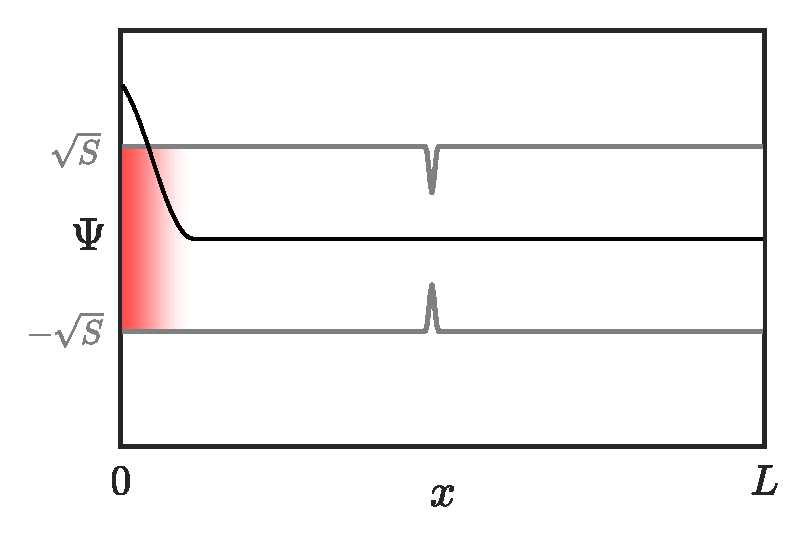
\includegraphics[width=\figWidth\textwidth]{figures/resonators/brass/websterPropagation1.eps}}\hfill
    \subfloat[$t = 5$ ms.\label{fig:websterPropagation2}]{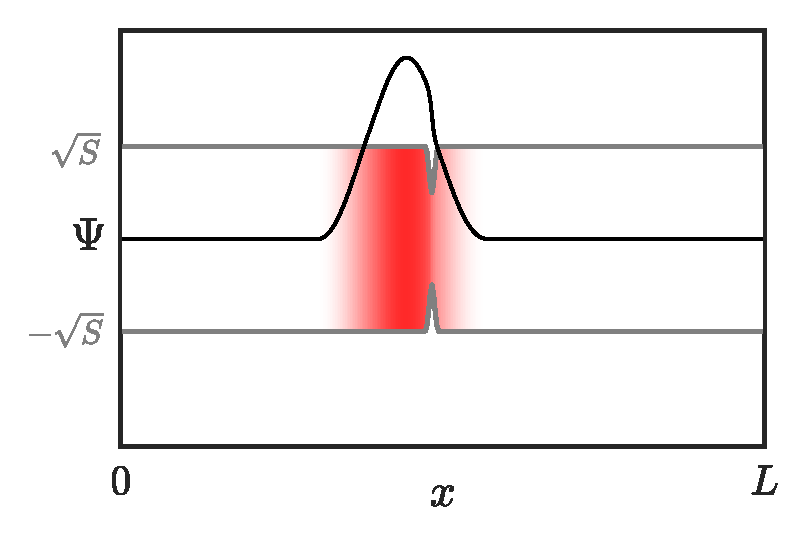
\includegraphics[width=\figWidth\textwidth]{figures/resonators/brass/websterPropagation2.eps}}\hfill
    \subfloat[$t = 8$ ms.\label{fig:websterPropagation3}]{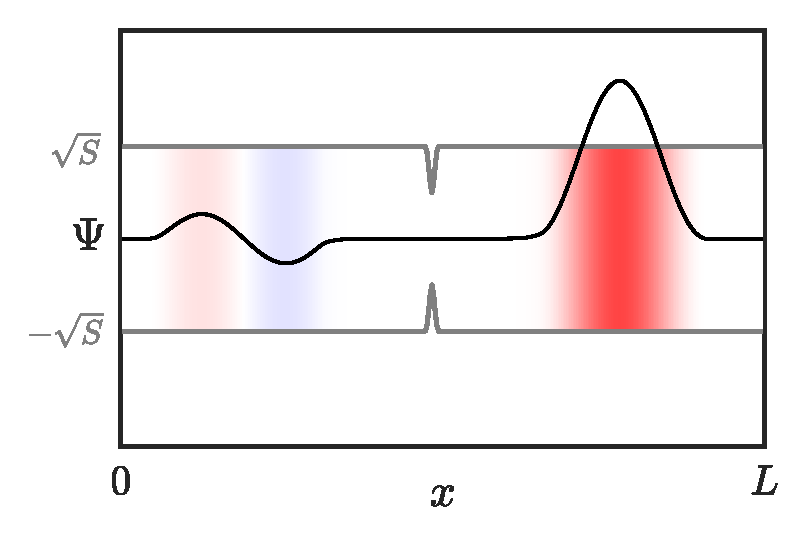
\includegraphics[width=\figWidth\textwidth]{figures/resonators/brass/websterPropagation3.eps}}
    \caption{Wave propagation and dispersion in an acoustic tube of varying cross-section (shown in grey) modelled by Webster's equation in Eq. \eqref{eq:webstersPDE}. Positive acoustic potential $\Psi$ is shown in red and negative in blue, which is also plotted for clarity. \label{fig:websterPropagation}}
\end{figure}
%test for git

\subsubsection{Boundary conditions}
The choices for boundary conditions in an acoustic tube are open and closed, defined as \cite{Bilbao2018}
\begin{subequations}\label{eq:contBoundariesBrass}
    \begin{align}
        \partial_t\Psi(0, t) &= 0, & \partial_t\Psi(L, t) &= 0, & &\text{(Dirichlet, open)},\label{eq:contDirichletBrass}\\
        \partial_x\Psi(0, t) &= 0, & \partial_x\Psi(L, t) &= 0, & &\text{(Neumann, closed)}\label{eq:contNeumannBrass}.
    \end{align}
\end{subequations}
This might be slightly counter-intuitive as when compared to the 1D wave equation, as ``closed" might imply the ``fixed" or Dirichlet boundary condition. The opposite can be intuitively shown by imagining a wave front with a positive acoustic potential (and thus positive pressure according to Eq. \eqref{eq:pressureVelocityWebster}) moving through a tube and hitting a closed end. What reflects is also a wave front with a positive acoustic potential, i.e., the sign of the potential does not flip. This also happens using the free or Neumann condition for the 1D wave equation (see Figure \ref{fig:boundaryCondsCont}).
Here, the following boundaries are chosen
\begin{equation}\label{eq:openClosed}
    \partial_x\Psi(0, t) = 0, \quad \text{and} \quad \partial_t\Psi(L, t) = 0,
\end{equation}
i.e. closed at the left end and open at the right end.

\subsection{Discrete time}
The state variable is discretised to the grid function $\Psi_l^n$ and is defined for $n\in \mathbb{N}^0$ and $l = \{0, \hdots, N\}$, where $N$ is the number of intervals between the grid points.
As the cross-section is distributed in space, $S(x)$ needs to be discretised to a grid function as well, albeit only in space (as it is not time-varying). Following \cite{Bilbao2018}, it is useful to introduce \textit{interleaved grid points} at $l-1/2$ and $l+1/2$ for $S$ and are defined as 
\begin{equation}\label{eq:sHalf}
    \Sm = \mxm S(x=lh), \qaq \Sp = \mxp S(x=lh),
\end{equation}
and approximate a `true' (possibly measured) bore profile $S(x)$ sampled at $x=lh$ with grid spacing $h$ (see Figure \ref{fig:variableCrossSection}). Using these definitions, one can discretise Eq. \eqref{eq:webstersPDE} to the following FD scheme \cite{theBible}\footnote{Notice that in \cite{theBible}, Webster's equation is $\Sbar_l \delta_{tt}\Psi^n_l = c^2\dxp(\Sm(\dxm\Psiln))$ but is identical to Eq. \eqref{eq:discWebster}. This discretisation has been chosen for a more straightforward energy analysis in Section \ref{sec:energyAnalysisWebster}.}
\begin{equation}\label{eq:discWebster}
    \Sbar_l \delta_{tt}\Psi^n_l = c^2\dxm\left(\Sp(\dxp\Psiln)\right),
\end{equation}
where
\begin{equation}\label{eq:Sbar}
    \Sbar_l = \mxp\Sm = \mxm\Sp = \mxx S(x=lh),
\end{equation}
the choice of which will become apparent in Section \ref{sec:stabilityEnergyWebster}.
The right-hand side of the scheme contains an operator applied to two grid functions ($S$ and $\Psi$) multiplied onto each other. In order to expand this, the product rule must be used. Recalling Eq. \eqref{eq:productRule} and applying this to backwards spatial operators instead yields
\begin{equation}
    \dxm (u_l^nw_l^n) = (\dxm u_l^n)(\mxm w_l^n) + (\mxm u_l^n)(\dxm w_l^n).
\end{equation}
Using the product rule, the right-hand side of Eq. \eqref{eq:discWebster} can be expanded to
\begin{equation*}
    \Sbar\dtt\Psiln = c^2\left[(\dxm \Sp)(\mxm (\dxp \Psiln)) + (\mxm \Sp)(\dxm (\dxp \Psiln))\right],
\end{equation*}
and solving for $\Psinp$ yields the following update equation (see Appendix \ref{app:webstersUpdateEq}):
\begin{equation}
    \Psinp = 2(1-\lambda^2)\Psiln-\Psinm+ \frac{\lambda^2\Sp}{\Sbar_l}\Psilp + \frac{\lambda^2\Sm}{\Sbar_l}\Psilm,\label{eq:webstersUpdateEq}
\end{equation}
with 
\begin{equation}
    \lambda = \frac{ck}{h},
\end{equation}
and similar to the 1D wave equation in Section \ref{sec:1DWaveDisc} needs to abide
\begin{equation}\label{eq:CFLwebster}
    \lambda \leq 1,
\end{equation}
in order for the scheme to be stable. See Section \ref{sec:stabilityEnergyWebster} for a derivation. The number of grid points $N$ can then be calculated in the same way as for the 1D wave equation in Eq. \eqref{eq:orderOfCalc}.

Notice that at the boundaries, Eq. \eqref{eq:webstersUpdateEq} requires values of $S$ (through its definition in Eq. \eqref{eq:Sbar}) outside of the defined domain, i.e., $S_{N+1/2}$ and $S_{-1/2}$. To solve this, one can set $\Sbar_0 = S(0)$ and $\Sbar_N = S(L)$ from which $S_{-1/2}$ and $S_{N+1/2}$ can be calculated according to
\begin{subequations}
    \begin{align}
        \Sbar_0 = \frac{1}{2}(S_{1/2} + S_{-1/2}) \ &\Rightarrow \ S_{-1/2} = 2\Sbar_0 - S_{1/2},\\
        \Sbar_N = \frac{1}{2}(S_{N+1/2} + S_{N-1/2}) \ &\Rightarrow \ S_{N+1/2} = 2\Sbar_N - S_{N-1/2}.\label{eq:Snph}
    \end{align} 
\end{subequations}
Although these values will not be needed when discretising the boundary conditions in Eq. \eqref{eq:contBoundariesBrass}, they will be useful at a later point.

\begin{figure}[t]
    \centering
    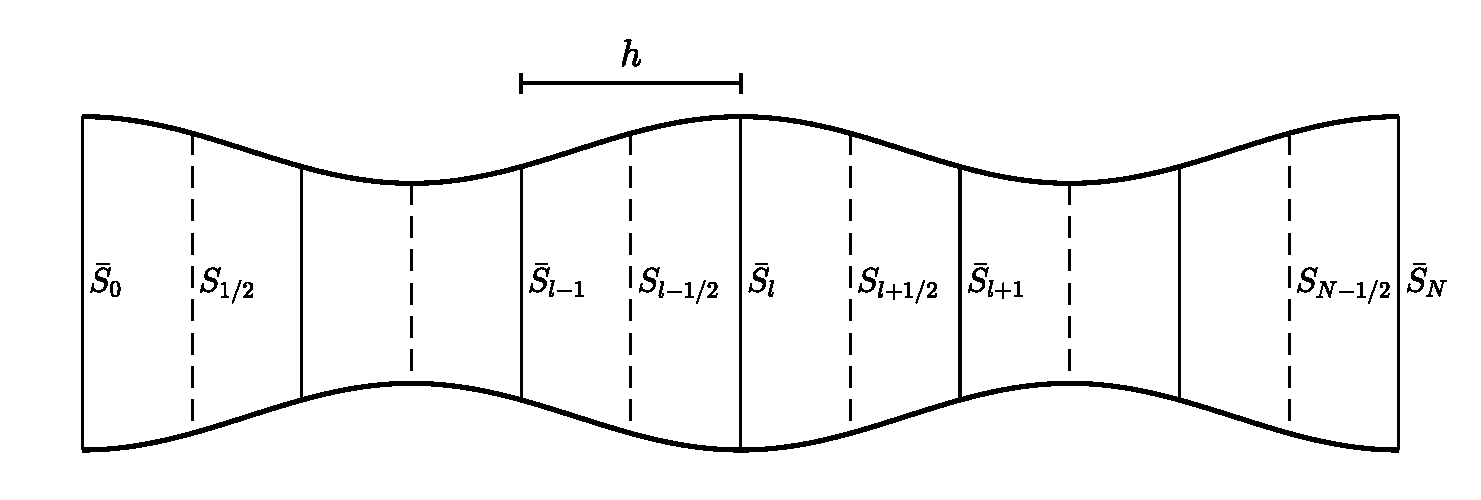
\includegraphics[width=0.9\textwidth]{figures/resonators/brass/variableCrossSection.eps}
    \caption{Approximations to $S(x)$ used in the FD scheme implementing Webster's equation. Dashed lines indicate the interleaved grid on which $S$ is sampled (Eq. \eqref{eq:sHalf}) and solid lines indicate $\Sbar$ which are averages of these (Eq. \eqref{eq:Sbar}). \label{fig:variableCrossSection}}
\end{figure}


\subsubsection{Boundary conditions}
One can discretise the continuous boundary conditions in Eq. \eqref{eq:openClosed} (closed at $x=0$, open at $x=L$) using centred difference operators for higher accuracy
\begin{subequations}\label{eq:discBoundariesBrass}
    \begin{align}
        \dxd\Psi_0^n &= 0 \quad \Rightarrow \quad\Psi_{-1}^n = \Psi_1^n ,\quad \!\!\!\!\!\!&&\text{(Neumann, closed)}, \label{eq:closedLeftBrass}\\
        \dtd\Psi_N^n &= 0\quad\Rightarrow \quad \Psi_N^n = 0, \quad \!\!\!\!\!\!&&\text{(Dirichlet, open)}\label{eq:openRightBrass}.
    \end{align}
\end{subequations} 
At the left boundary, Eq. \eqref{eq:webstersUpdateEq} can be expanded to:
\begin{equation*}
    \begin{aligned}
        \Psi_0^{n+1} &= 2(1-\lambda^2)\Psi_0^n-\Psi_0^{n-1}+ \frac{\lambda^2S_{1/2}}{\bar S_0}\Psi_1^n + \frac{\lambda^2S_{-1/2}}{\bar S_0}\Psi_{-1}^n,\\[-0.5em]
        \xLeftrightarrow{\mystrut\ \text{Eq. \eqref{eq:closedLeftBrass}}\ }\quad\Psi_0^{n+1} &= 2(1-\lambda^2)\Psi_0^n-\Psi_0^{n-1}+ \frac{\lambda^2(S_{1/2}+S_{-1/2})}{\bar S_0}\Psi_1^n,
    \end{aligned}
\end{equation*}
and as $\Sbar_0 = \frac{1}{2}(S_{1/2}+S_{-1/2})$ through Eq. \eqref{eq:Sbar}, this can be solved to
\begin{equation}\label{eq:leftBoundaryWebster}
    \Psi_0^{n+1} = 2(1-\lambda^2)\Psi_0^n-\Psi_0^{n-1}+ 2\lambda^2\Psi_1^n.
\end{equation}
One can implement the right boundary condition by simply reducing the range of operation to $l = \{0, \hdots, N-1\}$, as $\Psi_N^n = 0$ according to Eq. \eqref{eq:openRightBrass}. A more realistic boundary condition for the open end is presented in the following.

\subsection{Radiation}\label{sec:radiating}
One of the ways that an acoustic tube loses energy, is through radiation. The right boundary condition presented in Eq. \eqref{eq:openClosed} can be changed to be radiating according to \cite{theBible}
\begin{equation}\label{eq:radCont}
    \partial_x\Psi(L,t) = -a_1\partial_t\Psi(L,t)-a_2\Psi(L,t),
\end{equation}
where, for a tube terminating on an infinite plane \cite{Atig2004}
\begin{equation}
    a_1 = \frac{1}{2(0.8216)^2c}\ , \quad \text{and} \quad a_2 = \frac{L}{0.8216\sqrt{S_0S(1)/\pi}}\ ,
\end{equation}
which determine the amount of loss and inertia at the radiating boundary respectively. 

The radiating boundary in Eq. \eqref{eq:radCont} can then be discretised to \cite{theBible}
\begin{equation}\label{eq:centRadBound}
    \delta_{x\cdot}\Psi_N^n = -a_1\dtd\Psi_N^n - a_2\mu_{t\cdot}\Psi_N^n,
\end{equation}
which can be expanded and solved for $\Psi_{N+1}^n$ according to
\begin{equation}
    \Psi_{N+1}^n = h\left(-\frac{a_1}{k}(\Psi_N^{n+1} - \Psi_N^{n-1}) - a_2(\Psi_N^{n+1} + \Psi_N^{n-1})\right) + \Psi_{N-1}^n.
\end{equation}
Substitution into Eq. \eqref{eq:webstersUpdateEq} at the $l=N$ yields the following update equation
\begin{equation}
    \Psi_N^{n+1} = \frac{2(1-\lambda^2)\Psi_N^n-\Psi_N^{n-1}+\alpha_-\Psi_N^{n-1} + 2\lambda^2\Psi_{N-1}^n}{\left(1+\alpha_+\right)},
\end{equation}
where
\begin{equation}
    \alpha_\pm = h\left(\frac{a_1}{k}\pm a_2\right)\frac{\lambda^2S_{N+1/2}}{\bar S_N}.
\end{equation}
One can observe that $S_{N+1/2}$ is needed which is outside the defined domain. As mentioned before, setting $\Sbar_N = S(L)$, one can calculate $S_{N+1/2}$ using Eq. \eqref{eq:Snph} to solve the issue. 

\subsection{Excitation}\label{sec:webstersExcitation}
Although excitations will be discussed more in-depth in Part \ref{part:exciters}\todo{maybe refer to chapter/section instead}, a simple way to excite Webster's equation will be presented here.

Following \cite{Bilbao2018}, one can create an input signal $v_\text{in} = v_\text{in}(t)$ that interacts with the particle velocity of the tube. As this relates to the acoustic potential as in Eq. \eqref{eq:pressureVelocityWebster}, one can change the boundary condition of the left boundary to
\begin{equation}
    \px \Psi(0, t) = - v_\text{in}.
\end{equation}
Discretising this using the centred spatial operator yields
\begin{equation}
    \dxd \Psi_0^n = -v_\text{in}^n \quad \Rightarrow \quad \Psi_{-1}^n = 2h v_\text{in}^n + \Psi_1^n,
\end{equation}
and can be substituted into the update equation in Eq. \eqref{eq:webstersUpdateEq} at $l=0$ to get
\begin{align}
    \Psi_0^{n+1} &= 2(1-\lambda^2)\Psi_0^n-\Psi_0^{n-1} \frac{\lambda^2S_{1/2}}{\Sbar_0}\Psi_1^n + \frac{\lambda^2S_{-1/2}}{\Sbar_0}\left(2h v_\text{in}^n + \Psi_1^n\right),\nonumber\\
    \Psi_0^{n+1} &= 2(1-\lambda^2)\Psi_0^n-\Psi_0^{n-1} +2\lambda^2\Psi_1^n + \frac{2h\lambda^2S_{-1/2}}{\Sbar_0} v_\text{in}^n.
\end{align}
The input signal is arbitrary, but looking towards lip excitation, and following \cite{theBible}, one can set the input to a pulse train as shown in Figure \ref{fig:inputWebster}. More details can be found in Chapter \ref{ch:physInspExcitations}.
\begin{figure}[h]
    \centering
    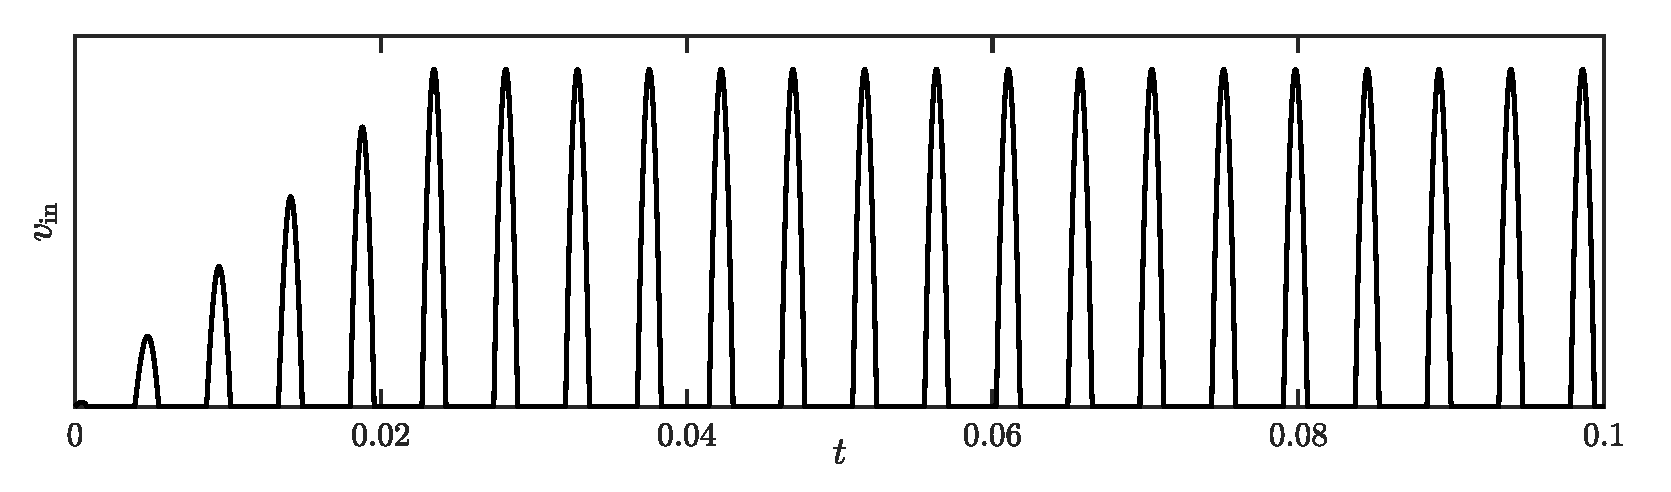
\includegraphics[width=\textwidth]{figures/resonators/brass/inputWebster.eps}
    \caption{A pulse train with a frequency of $213$ Hz. This is used to excite the implementation of Webster's equation in Section \ref{sec:outputWebster}. \label{fig:inputWebster}}
\end{figure}

% At the left boundary, one can sed $\bar S_N = S_N$ from which $S_{N+1/2}$ can be calculated:
% \begin{equation}
%     S_N = \frac{1}{2}(S_{N+1/2} + S_{N-1/2}) \ \Rightarrow \ S_{N+1/2} = 2S_N - S_{N-1/2}.
% \end{equation}
% % \begin{equation}
% %         S_0 = \frac{1}{2}(S_{1/2} + S_{-1/2}) \ \Rightarrow \  S_{-1/2}
% %         = 2S_0 - S_{1/2}
% % \end{equation}



% The same can be done for the right boundary ($\bar S_N = S_N$) if this is chosen to be anything else but open (e.g., closed or radiating -- see Section \ref{sec:radiating}):
% \begin{equation}
%     S_N = \frac{1}{2}(S_{N+1/2} + S_{N-1/2}) \ \Rightarrow \ S_{N+1/2} = 2S_N - S_{N-1/2}.
% \end{equation}
% For now though, we follow the conditions given in \eqref{eq:openClosed} and we can simply set the right boundary to its initial state
% \begin{equation}
%     \Psi_N^n = \Psi_N^0
% \end{equation}
% which is normally $0$. A more realistic open end is a radiating one, which can be found below.

\subsection{Matrix form and output}\label{sec:outputWebster}
One can write scheme \eqref{eq:discWebster} in matrix form by saving the state in a vector $\boldPsi^n = [\Psi_0^n, \hdots, \Psi_N^n]^T$ and creating a $\Dxx$ matrix that includes the effect of the cross-sectional area $S$. Assuming Neumann boundary conditions yields
\begin{equation}
    \Dxx = \frac{1}{h^2}\begin{bmatrix}
        -2& 2 &  & & & \mathbf{0}& \\
        \frac{S_{1/2}}{\Sbar_1} & -2 &\frac{S_{3/2}}{\Sbar_1} & & & & \\
        & \ddots & \ddots & \ddots &  & & \\
        & & \frac{S_{l-1/2}}{\Sbar_l}& -2 & \frac{S_{l+1/2}}{\Sbar_l} & & \\
        & & & \ddots & \ddots & \ddots & \\
        & & &  & \frac{S_{N-3/2}}{\Sbar_{N-1}}  & -2 & \frac{S_{N-1/2}}{\Sbar_{N-1}} \\
        & \mathbf{0} & & & & 2 & -2 \\
    \end{bmatrix}.
\end{equation}
Notice that there are no appearances of $S$ at the boundaries as these vanish due to the boundary conditions as in Eq. \eqref{eq:leftBoundaryWebster}.
Using $\I_N$ as the $N\times N$ identity matrix, one can write scheme \eqref{eq:discWebster} in matrix form as
\begin{equation}\label{eq:matrixFormWebsters}
    \A\boldPsi^{n+1} = \B\boldPsi^n + \C \boldPsi^{n-1} + \mathbf{v}^n
\end{equation}
where 
\begin{equation*}
    \begin{gathered}
    \A = \begin{bmatrix}
        \I_{N}& \mathbf{0}\\\
        \mathbf{0} & 1 + \alpha_+\
    \end{bmatrix}, \quad \B = 2\I + c^2 k^2 \Dxx, \quad \text{and} \quad \C = \begin{bmatrix}
        -\I_N & \mathbf{0}\\\
        \mathbf{0}& -1 + \alpha_-
    \end{bmatrix},
    \end{gathered}
\end{equation*}
and the $(N+1)\times 1$ input vector $\mathbf{v}^n$ consists of zeros except for the first index:
\begin{equation}
    \mathbf{v}_i^n = 
    \begin{cases}
        \frac{2h \lambda^2 S_{-1/2}}{\Sbar_0}v_\text{in}^n, & \text{if } i = 1,\\
        0,& \text{otherwise}.
    \end{cases}
\end{equation}
%
Notice how the radiation is included by changing the last entry of matrices $\A$ and $\C$.
The output of an implementation of Webster's equation is shown in Figure \ref{fig:outputWebster}. The parameters used for the scheme, the input signal and the geometry used to obtain the output can be found in Table \ref{tab:websterParams}, Figure \ref{fig:inputWebster}, and Figure \ref{fig:geometryWebster} respectively.
\begin{figure}[h]
    \centering
    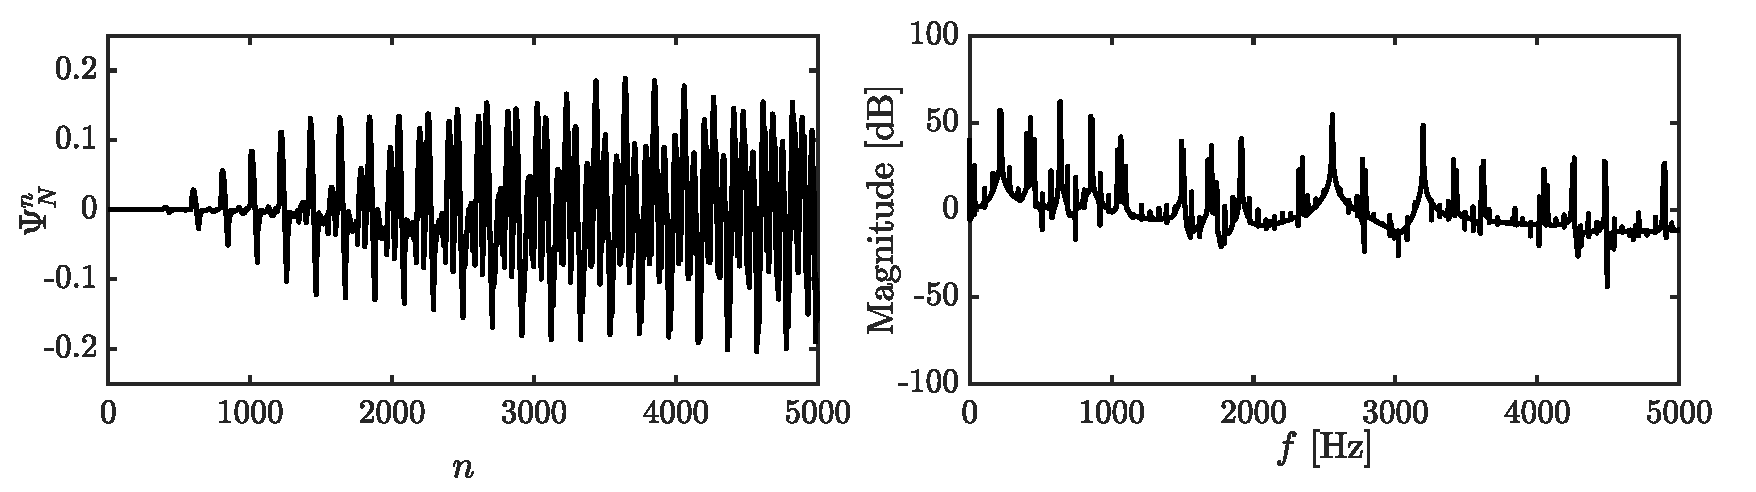
\includegraphics[width=\textwidth]{figures/resonators/brass/outputWebster.eps}
    \caption{The output of Webster's equation at $\Psi_N^n$ using the parameters in Table \ref{tab:websterParams} and geometry in Figure \ref{fig:geometryWebster}. \label{fig:outputWebster}}
\end{figure}

\begin{table}[h]
    \begin{center}
    \begin{tabular}{|l|c|c|}
        \hline
        Name & Symbol (unit) & Value\\ \hline
        Length & $L$ (m) & $\approx 3$\\
        Wave speed & $c$ (m/s) & 343\\
        Cross-sectional area & $S(x)$ & See e.g. paper \citeP[H]\\\hline
        \end{tabular}
    \caption{Parameters for the implementation of Webster's equation. The length is slightly below $3$ m to yield $\lambda = 1$ in Eq. \eqref{eq:CFLwebster}.\label{tab:websterParams}}
    \end{center}
\end{table}
{\renewcommand{\arraystretch}{1}

\hspace{0.1\textwidth}
\begin{figure}[h]
    \centering
    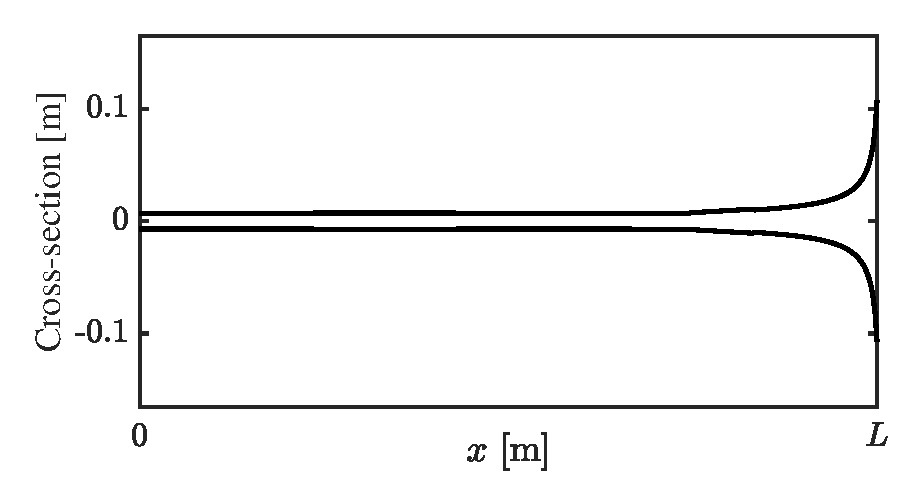
\includegraphics[width=0.6\textwidth]{figures/resonators/brass/geometryWebster.eps}
    \caption{The geometry used for the implementation. See paper \citeP[H] for more details. \label{fig:geometryWebster}}
\end{figure}


\subsection{Energy analysis}\label{sec:energyAnalysisWebster}
The energy analysis of Webster's equation with a radiating boundary might seem straightforward. However, due to the varying cross-sectional area, the energy balance deserves a more detailed treatment, especially at the boundaries. For this analysis, (centred) Neumann boundary conditions are used for both boundaries and the input is ignored. This section follows the steps presented in Section \ref{sec:energyAnalysis}.% to retain generality. %These can then easily be adapted to Dirichlet if needed.

\subsubsection{Step 1: Obtain $\dtp \h$}
Usually, to ensure vanishing boundary terms when using centred Neumann boundary conditions, the primed inner product in Eq. \eqref{eq:primedInnerProd} is chosen. However, as the system has a spatially varying cross-section, the more general \textit{weighted inner product} in Eq. \eqref{eq:weightedInnerProd} has to be chosen instead.

Taking an inner product weighted by free parameters $0 < \el, \er \leq 2$ at the left and right boundary respectively, of scheme \eqref{eq:discWebster} with $(\dtd \Psiln)$ over discrete domain $d$ yields 
\begin{equation}\label{eq:powerBalanceWebster}
    \dtp \h = \langle \dtd\Psiln ,\Sbar_l \delta_{tt}\Psi^n_l\rangle_d^{\el,\er} - c^2\langle\dtd\Psiln, \dxm(\Sp(\delta_{x+}\Psiln))\rangle_d^{\el,\er} = 0.
\end{equation}

\subsubsection{Step 2: Identify energy types and isolate $\dtp$} 
As the right boundary is set to be radiating according to Eq. \eqref{eq:centRadBound}, the energy balance will eventually be of the following form:
\begin{equation}\label{eq:radiatingEnergyForm}
    \delta_{t+}(\mathfrak{h}+\mathfrak{h}_\text{b}) = \b-\mathfrak{q}_\text{b},
\end{equation}
where $\mathfrak{h}_\text{b}$ is the energy stored by the radiating boundary through the inertia term, $\mathfrak{q}_\text{b}$ describes the the energy losses through radiation and $\b$ is the general boundary term.

% As one can rewrite
% \begin{equation}\label{eq:switchSignsWebster}
%     \dxp\left(\Sm(\delta_{x-}\Psiln)\right) \ \Longleftrightarrow\  \dxm\big(\Sp(\dxp\Psiln)\big),
% \end{equation}
Starting at Eq. \eqref{eq:powerBalanceWebster}, the last term can -- using identity \eqref{eq:weightedIdentityMinus} -- be rewritten to
\begin{equation*}
    c^2\langle\Sp \dtd \dxp \Psiln, (\dxp \Psiln)\rangle_{\underline{d}} + \b_\text{r} - \b_\text{l},
\end{equation*}
where
\begin{subequations}
    \begin{align}
     \mathfrak{b}_\text{r} &= c^2(\dtd\Psi_N^n)\left(\frac{\epsilon_\text{r}}{2}S_{N+1/2}(\dxp \Psi_N^n) + \left(1-\frac{\epsilon_\text{r}}{2}\right)S_{N-1/2}(\dxm\Psi_N^n)\right), \\
     \mathfrak{b}_\text{l} &= c^2(\dtd\Psi_0^n)\left(\frac{\epsilon_\text{l}}{2}S_{-1/2}(\dxm\Psi_0^n)+\left(1-\frac{\epsilon_\text{l}}{2}\right)S_{1/2}(\dxp \Psi_0^n))\right),
    \end{align}
\end{subequations}
are the right and left boundary term respectively (notice that $\b_\text{l}$ is subtracted). One can immediately observe that the boundary terms vanish if Dirichlet boundary conditions would be used. 
    
Then, using identities \eqref{eq:prodIdentity1} and \eqref{eq:prodIdentity2} yields 
\begin{equation*}
    \dtp \h = \b_\text{r} - \b_\text{l}
\end{equation*}
where
\begin{equation}\label{eq:energyBalanceWebster}
    \begin{gathered}
        \h = \t + \v, \qwiq \t = \frac{1}{2} \left(\lVert\sqrt{\Sbar_l} \dtm \Psiln \rVert_d^{\el, \er}\right)^2 \quad \text{and} \\
        % \v =c^2\langle\dtd \dxp \Psiln, \Sp(\dxp \Psiln)\rangle_{\underline{d}}\ .
        \v = \frac{c^2}{2}\langle \Sp\dxp \Psiln, e_{t-}\dxp\Psiln\rangle_{\underline{d}}
    \end{gathered}
\end{equation}
Notice that $\Sbar_l$ is included in the norm by using its square-root.

The next step is to find definitions for $\el$ and $\er$ such that the boundary terms vanish if radiation were to be ignored. In other words, the boundary terms need to be rewritten such that 
\begin{align*}
    \dxd \Psi_0^n &= 0\  \Rightarrow\ \b_\text{l} = 0 \\
    \dxd \Psi_N^n &= 0\  \Rightarrow\ \b_\text{r} = 0
\end{align*} 
for the left and right boundary respectively. It can be shown that, for the special cases of $\epsilon_\text{r} = S_{N-1/2}/\mu_{xx}S_N$ and $\epsilon_\text{l} = S_{1/2}/\mu_{xx}S_0$ the boundary terms vanish in this case
\begin{subequations}\label{eq:centStrictDissip}
\begin{align}
    \mathfrak{b}_\text{r} &= c^2 (\dtd\Psi_N^n)S_{N-1/2}(2-\epsilon_\text{r})(\delta_{x\cdot}\Psi_N^n)\label{eq:centStrictDissipRight},\\
    \mathfrak{b}_\text{l} &= c^2 (\dtd\Psi_0^n)S_{1/2}(2-\epsilon_\text{l})(\delta_{x\cdot}\Psi_0^n).\label{eq:centStrictDissipLeft}
\end{align}
\end{subequations}
See Appendix \ref{app:boundaryWebster} for a derivation of this. %Also note that $\el, \er \leq 2$ to the boundary terms to be non-negative. 

To add the energy stored and dissipated by the radiating boundary, its definition in Eq. \eqref{eq:centRadBound} can be substituted into the right boundary term $\b_\text{r}$ in Eq. \eqref{eq:centStrictDissipRight} as 
\begin{align*}
    \mathfrak{b}_\text{r} &= c^2 (\dtd\Psi_N^n)S_{N-1/2}(2-\epsilon_\text{r})(-a_1\dtd\Psi_N^n - a_2\mu_{t\cdot}\Psi_N^n),\\
    &= c^2 S_{N-1/2}(2-\epsilon_\text{r})\left(-a_1(\dtd\Psi_N^n)^2 - a_2(\dtd\Psi_N^n)(\mu_{t\cdot}\Psi_N^n)\right).
\end{align*}
This can then be decomposed in $\h_\text{b}$ and $\q_\text{b}$ used in Eq. \eqref{eq:powerBalanceWebster}. 
% These can be obtained by substituting the definition of the radiating boundary Eq. \eqref{eq:centRadBound} into \eqref{eq:centStrictDissipRight} to get

Using identity \eqref{eq:prodIdentity4} -- and identity \eqref{eq:identity2} thereafter -- yields the definitions for $\h_\text{b}$ and $\q_\text{b}$ in Eq. \eqref{eq:radiatingEnergyForm}
\begin{equation}
    \h_\text{b} = \frac{c^2 S_{N-1/2}(2-\epsilon_\text{r}) a_2}{2} \mtm(\Psi_N^n)^2, \qaq \q_\text{b} = c^2 S_{N-1/2}(2-\epsilon_\text{r})a_1(\dtd\Psi_N^n)^2.
\end{equation}
Finally, $\b = \b_\text{l}$ and can be shown to vanish for both Dirichlet and (centred) Neumann conditions.

\subsubsection{Step 3: Check units}
\SWcomment[It seems like in order for the units to make sense, one must write Eq. \eqref{eq:webstersPDE} as
\begin{equation}
    \frac{S\rho}{c^2} \ptt\Psi = \frac{B}{c^2}\px(S(\px\Psi)),
\end{equation}
where $B$ is the bulk modulus of air (in N/m$^2$)]
\subsubsection{Step 4: Implementation}
Figure \ref{fig:energyWebsters} shows the energetic output of Webster's equation with a radiating boundary at $x=L$. To highlight the effect of the radiation on the energy the parameters are set to $L = 1$ and $S(x) = 0.01$ for all $x\in \D$.  The system is excited with a raised cosine close to the left boundary, and when the excitation reaches the radiating boundary, the total energy in the system decreases due to the losses. The energy stored by the boundary $\h_\text{b}$ is also shown and indeed increases when the wave reaches the boundary.
\begin{figure}[h]
    \centering
    \begin{tikzpicture}[->,node distance=3cm,
        thick,main node/.style={circle,draw}]
    
        \node[] (image) at (0,0) {
        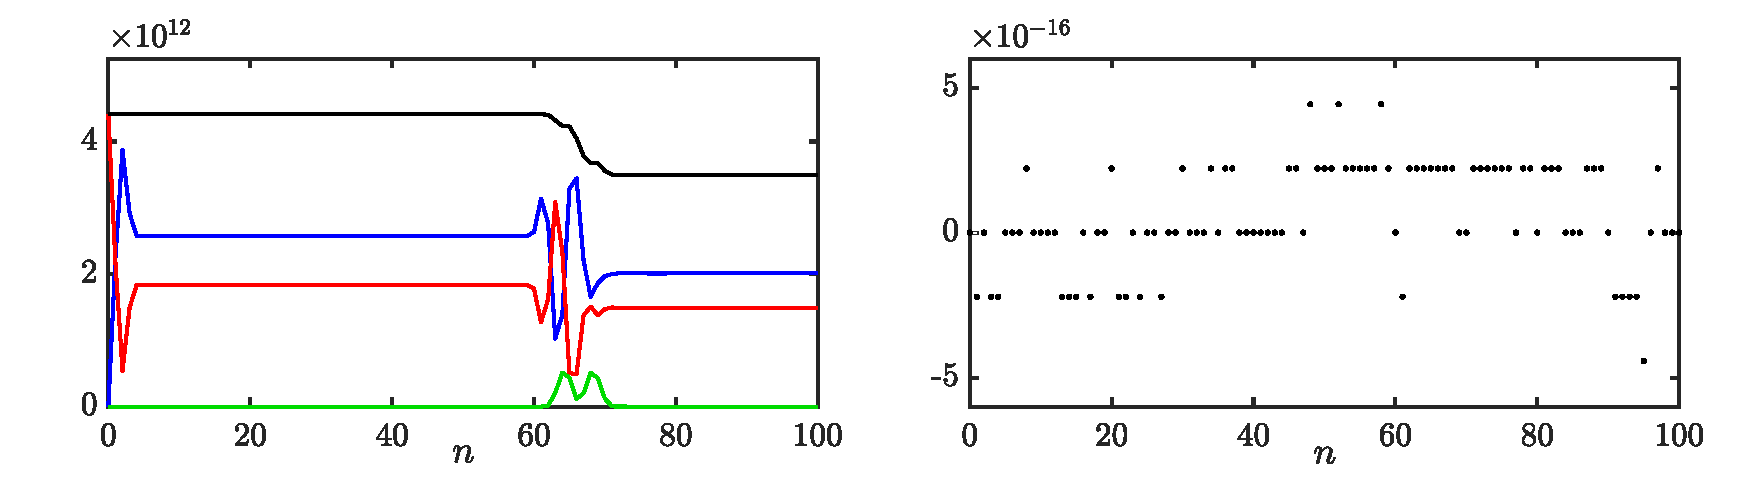
\includegraphics[width=\textwidth]{figures/resonators/brass/energyWebster2.eps}
        };
    
        \node[] (he) at (0.2,0.5) {\small $\mathfrak{h}_\text{e}$};

        \node[] (h) at (-5.75, 1) {\small $\mathfrak{h}$};
        \node[] (v) at (-5.75, 0.5) {\small $\color{red}\mathfrak{v}$};
        \node[] (t) at (-5.75, 0) {\small $\color{blue}\mathfrak{t}$};
        \node[] (hb) at (-5.75, -0.5) {\small $\color[HTML]{00DB00}\mathfrak{h}_\text{b}$};      
    \end{tikzpicture}
      \caption{The kinetic (blue), potential (red), and total (black) energy as well as the energy stored by the radiation condition (green) of an implementation of Webster's equation are plotted in the left panel. Notice that the energy decreases between $n=60$ and $n=70$ as the excitation reached the boundary where damping is included. The right panel shows the normalised energy (according to Eq. \eqref{eq:normalisedEnergyDamping}) and shows that the deviation of the energy is within machine precision. \label{fig:energyWebsters}}
\end{figure}

\subsection{Stability through energy analysis}\label{sec:stabilityEnergyWebster}
Frequency domain analysis as presented in Section \ref{sec:stabilityAnalysis}, or more specifically, von Neumann analysis, can not be performed on Webster's equation due to the varying cross-section of the system \cite{theBible}. Instead, stability conditions can be obtained through energy analysis explained in Section \ref{sec:stabilityAnalysisEnergy}.

Consider the following scheme
\begin{equation}
    [S]_l \delta_{tt}\Psi^n_l = c^2\dxm(\Sp(\delta_{x+}\Psiln)),
\end{equation}
where $[S]_l$ is a still undetermined second-order approximation to the true geometry of the acoustic tube and will be shown to be $\Sbar_l$ below. As done for the 1D wave equation in Section \ref{sec:stabilityAnalysisEnergy}, the potential energy $\v$ in Eq. \eqref{eq:energyBalanceWebster} can be rewritten using identity \eqref{eq:prodIdentityEnergyStab} as
\begin{equation*}
    \v = \frac{c^2}{2}\left(\lVert\sqrt{S_{l+1/2}}\mtm\dxp\Psiln\rVert_{\underline{d}}^2-\frac{k^2}{4}\lVert\sqrt{S_{l+1/2}}\dtm\dxp \Psiln\rVert_{\underline{d}}^2\right).
\end{equation*}
For spatially varying systems, one can use the following extension of the bound given in Eq. \eqref{eq:spatialBound} \cite{theBible}
\begin{equation}\label{eq:spatialBoundWebster}
    \lVert \sqrt{\phi_l}\dxp \uln \rVert_{\underline{d}} \leq\frac{2}{h}\lVert \sqrt{\mxm\phi_l} \uln \rVert_d,
\end{equation}
where spatially varying function $\phi_l > 0$ is defined over the same domain as $u$. The following condition can then be put on $\v$
\begin{align*}
    \v &\geq \frac{c^2}{2}\left(\lVert\sqrt{S_{l+1/2}}\mtm\dxp\Psiln\rVert_{\underline{d}}^2 - \frac{k^2}{4}\left(\frac{2}{h}\lVert\sqrt{\mxm \Sp}\dtm\Psiln\rVert_{d}\right)^2\right),\\
    &\geq \frac{c^2}{2}\left(\lVert\sqrt{S_{l+1/2}}\mtm\dxp\Psiln\rVert_{\underline{d}}^2 - \frac{k^2}{h^2}\lVert\sqrt{\mxx S_l}\dtm\Psiln\rVert_{d}^2\right)\\
    & \geq \frac{c^2}{2}\left(\lVert\sqrt{S_{l+1/2}}\mtm\dxp\Psiln\rVert_{\underline{d}}^2 - \frac{k^2}{h^2}\left(\lVert\sqrt{\mxx S_l}\dtm\Psiln\rVert_{d}^{\el,\er}\right)^2\right),
\end{align*}
where last step is possible because $0 < \el, \er \leq 2$.
% Assuming that $\el, \er \leq 2$, the following is true
% \begin{equation}
%     \lVert \uln \rVert^{\el, \er}_d\leq \lVert \uln\rVert_d
% \end{equation}
% \begin{equation}
%     \t \geq 
% \end{equation}
Substituting this into the energy balance in Eq. \eqref{eq:energyBalanceWebster} yields
\begin{align*}
    \h = \t + \v \geq &\  \frac{1}{2} \left(\lVert\sqrt{[S]_l} \dtm \Psiln \rVert_d^{\el, \er}\right)^2 \\
    &+ \frac{c^2}{2}\left(\lVert\sqrt{S_{l+1/2}}\mtm\dxp\Psiln\rVert_{\underline{d}}^2 - \frac{k^2}{h^2}\left(\lVert\sqrt{\mxx S_l}\dtm\Psiln\rVert_{d}^{\el,\er}\right)^2\right),
\end{align*}
and as $\lVert\sqrt{S_{l+1/2}}\mtm\dxp\Psiln\rVert_{\underline{d}}^2$ is non-negative, the following is also true
\begin{equation*}
    \h = \t + \v \geq \frac{1}{2} \left(\lVert\sqrt{[S]_l} \dtm \Psiln \rVert_d^{\el, \er}\right)^2- \frac{\lambda^2}{2}\left(\lVert\sqrt{\mxx S_l}\dtm\Psiln\rVert_{d}^{\el,\er}\right)^2.
\end{equation*}
This can be written as
\begin{equation}
    \h \geq \frac{1}{2} \sum_d \left(\sqrt{[S]_l} - \lambda^2\sqrt{\mxx S_l}\right)(\dtm \Psiln)^2 
\end{equation}
which is non-negative if
\begin{align*}
    \text{min}\Big(\sqrt{[S]_l} - \lambda^2\sqrt{\mxx S_l}\Big) \geq 0,\\
    \lambda \leq \text{min}\left(\sqrt{\frac{[S]_l}{\mxx S_l}}\right).
\end{align*}
For the special choice of $[S]_l = \mxx S_l$, this condition reduces to
\begin{equation}
    \lambda \leq 1,
\end{equation}
also given in \eqref{eq:CFLwebster}. This choice of $[S]_l$ is equal to $\Sbar_l$ through Eq. \eqref{eq:Sbar}, hence its choice in Eq. \eqref{eq:discWebster}.

\subsection{Modal analysis}
The variable cross-section causes the modes of the system to vary in interesting ways. If the tube is perfectly cylindrical and $S(x)$ is thus constant, Webster's equation reduces to the 1D wave equation and the modal frequencies are integer multiples of the fundamental frequency. 
For low cross-sectional variations, the modes generally follow a linear pattern. See Figure \ref{fig:webstersModes}. The damping per mode, however, follows a different pattern, where higher damping occurs around $\fs/4$, and is due to the comb-filtering effect that the radiation has on the system. \SWcomment[is this true?]

\begin{figure}[h]
    \centering
    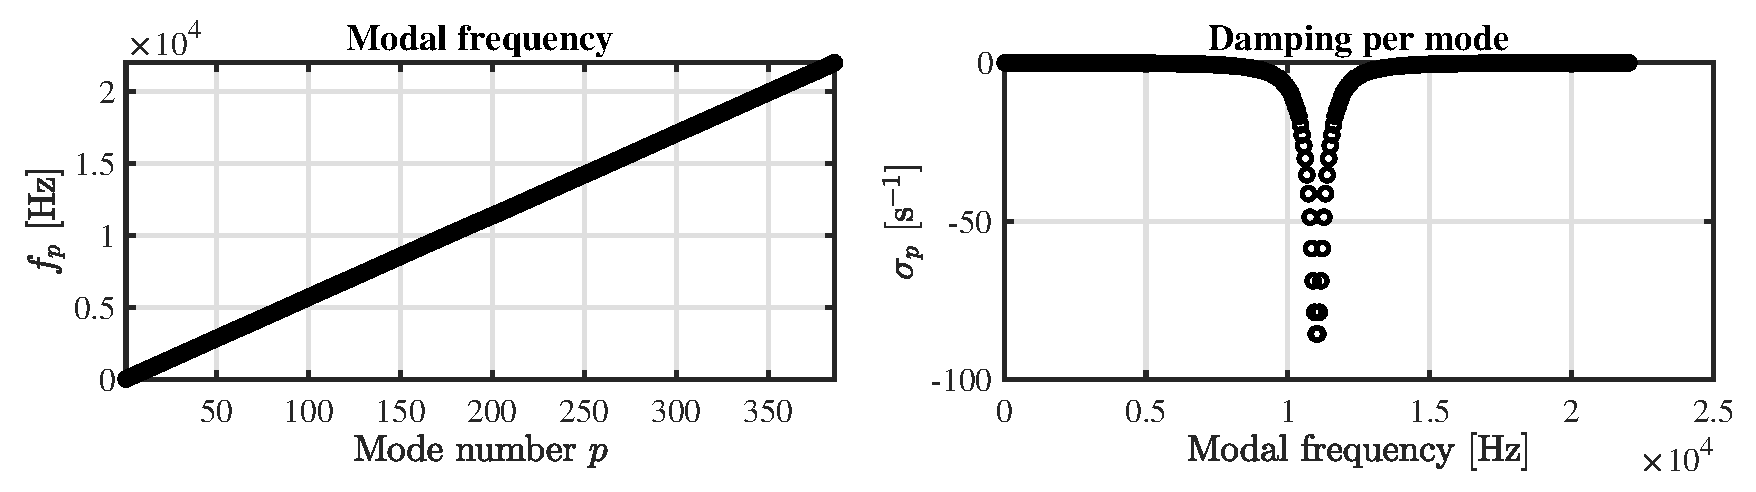
\includegraphics[width=\textwidth]{figures/resonators/brass/webstersModes.eps}
    \caption{The result of a modal analysis of Webster's equation with parameters and geometry given in \ref{sec:outputWebster}. Notice the higher damping for modes around $\fs/4$. \label{fig:webstersModes}}
\end{figure}

\section{First-order system}\label{sec:firstOrderSystem}
Until now, only PDEs  have been presented that second-order in time, i.e., that are dependent on the acceleration of the state variable. This section presents a system of two coupled first-order PDEs which are instead dependent on the velocity. State-of-the-art research on brass instruments in the context of FDTD methods also uses this coupled system (see e.g.\cite{Bilbao2016, Harrison2018}) and has been used in this project to model the trombone in paper \citeP[H].\todo{look at wording}

\subsection{Continuous time}
Using the same variables as before for cross-sectional area $S=S(x)$, wave speed $c$, and air density $\rho_0$, a system of PDEs that describes air propagation in an acoustic tube can be defined as follows:
\begin{subequations}\label{eq:firstOrderSystem}
\begin{align}
    \frac{S}{\rho_0 c^2}\partial_t p &= -\partial_x(Sv),\label{eq:contPressure}\\
    \rho_0\partial_tv &= -\partial_xp\label{eq:discVelocity},
\end{align}
\end{subequations}
where pressure $p = p(x,t)$ (Pa) and particle velocity $v = v(x,t)$ (m/s) are defined for $x\in \D$ with domain $\D = [0, L]$ and tube length $L$ (in m). These state variables are related to the acoustic potential $\Psi$ as shown in Eq. \eqref{eq:pressureVelocityWebster} as
\begin{equation}\label{eq:pressureVelocityFirstOrder}
    p = \rho_0\partial_t \Psi, \quad v = -\partial_x\Psi.
\end{equation}  
Indeed it can be shown by substituting these definitions into Eq. \eqref{eq:contPressure}, Webster's equation can be obtained:
\begin{equation}
  \nonumber
        \frac{S}{\rho_0 c^2}\partial_t(\rho_0 \partial_t\Psi) = -\partial_x(S(-\partial_x\Psi))\quad \Longrightarrow \quad S\partial_t^2\Psi = c^2\partial_x(S\partial_x\Psi).
\end{equation}


\subsubsection{Boundary conditions}
For the first-order PDE system in Eq. \eqref{eq:firstOrderSystem}, the boundary conditions are defined as follows:
\begin{subequations}
    \begin{align}\label{eq:firstOrderBoundaryConditionsCont}
        p(0,t) &= 0, &  p(L,t) &= 0, & &\quad\text{(Dirichlet, open)},\\
        S(0)v(0) &= 0, & S(L)v(L) &= 0, & &\quad \text{(Neumann, closed)},
    \end{align}
\end{subequations}
which, through Eq. \eqref{eq:pressureVelocityFirstOrder}, relate to the boundary conditions of Webster's equation in Eq. \eqref{eq:contBoundariesBrass}.

\subsection{Discrete time}
It is useful to place either $p$ or $v$ on an interleaved grid (see Figure \ref{fig:interleavedGrid}). Following \cite{Harrison2018}, $v$ is placed on this interleaved grid both in space and time. 
Accordingly, system \eqref{eq:firstOrderSystem} is discretised as
\begin{subequations}\label{eq:firstOrderFDS}
    \begin{align}
        \frac{\bar S_l}{\rho_0 c^2}\delta_{t+}p_l^n &= -\delta_{x-}(S_{l+1/2}v_{l+1/2}^{n+1/2}),\label{eq:discPressure}\\
        \rho_0 \delta_{t-}v_{l+1/2}^{n+1/2}&=-\delta_{x+}p_l^n,\label{eq:discVelocity}
    \end{align}
\end{subequations}
after which the update equations become
\begin{subequations}
    \begin{align}
        p_l^{n+1} &= p_l^n - \frac{\rho_0 c \lambda}{\bar{S}_l}(S_{l+1/2}v_{l+1/2}^{n+1/2}-S_{l-1/2}v_{l-1/2}^{n+1/2}),\label{eq:pressureUpdate}\\
        v_{l+1/2}^{n+1/2} &= v_{l+1/2}^{n-1/2}-\frac{\lambda}{\rho_0 c}(p_{l+1}^n - p_l^n),\label{eq:velocityUpdate}
    \end{align}
\end{subequations}
where (again) $\lambda = ck/h \leq 1$ for stability. The pressure is defined for $l=\{0, \hdots, N\}$ and the velocity for $l=\{0, \hdots, N-1\}$ where $N$ is the number of intervals between the grid points on the pressure grid. Notice that the range of calculation for the particle velocity is one fewer grid point than the that of the pressure.

An advantage of using an interleaved grid like this, is that the forward and backward first-order are second-order accurate, and can be shown through a Taylor series expansion as done in \ref{sec:FDoperators} (also see \cite{Harrison2018}).

\begin{figure}
    \centering
    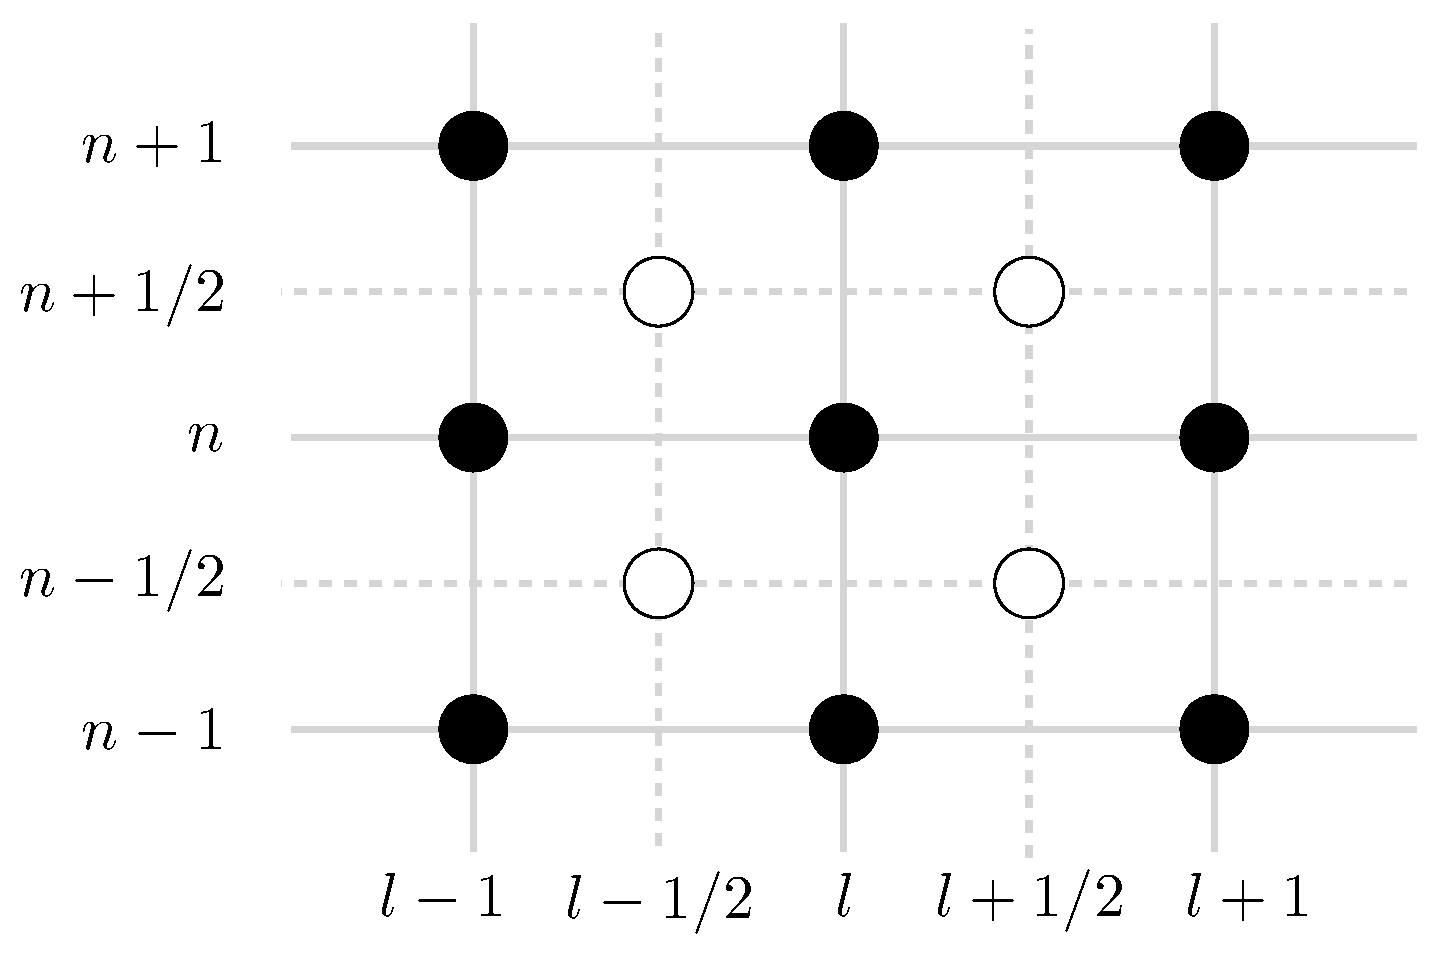
\includegraphics[width=0.7\textwidth]{figures/resonators/brass/interleavedGridFigure.pdf}
    \caption{The interleaved grid used for the system of FD schemes in Eq. \eqref{eq:firstOrderFDS}. Grid points on the regular grid (in black) are used for pressure $p$, while points on the interleaved grid (in white) are used for particle velocity $v$.\label{fig:interleavedGrid}}
\end{figure}

\subsubsection{Boundary conditions}\label{sec:boundariesFirstOrder}
The boundary conditions in Eq. \eqref{eq:firstOrderBoundaryConditionsCont} can be discretised as follows
\begin{subequations}
    \begin{align}\label{eq:firstOrderBoundaryConditions}
        p_0^n &= 0, & p_N^n &= 0, & &\text{(Dirichlet, open),}\\
        \mu_{x-}(S_{1/2}v_{1/2}^n) &= 0, & \mu_{x+}(S_{N-1/2}v_{N-1/2}^n) &= 0, & &\text{(Neumann, closed)}.
    \end{align}
\end{subequations}

\subsection{Matrix form}
System \eqref{eq:firstOrderFDS} can be written in matrix form, by saving the states of $p_l^n$ and $v_{l+1/2}^{n+1}$ in vectors as 
\begin{equation}
    \mathbf{p}^n = [p_0^n, \hdots, p_N^n]^T, \qaq \mathbf{v}^{n+1/2} = [v_{1/2}^{n+1/2}, \hdots, v_{N-1/2}^{n+1/2}]^T
\end{equation}
which are of sizes $(N+1)\times 1$ and $N\times 1$ respectively. One may then write the scheme in matrix form as  
\begin{subequations}
    \begin{align}
        \mathbf{v}^{n+1/2} &= \mathbf{v}^{n-1/2} + \B_p \mathbf{p}^n\\
        \mathbf{p}^{n+1} &= \mathbf{p}^n + \B_v \mathbf{v}^{n+1/2} 
    \end{align}
\end{subequations}
where
\begin{equation}
    \B_v = \frac{\rho_0 c}\lambda \begin{bmatrix}
        -\frac{2S_{1/2}}{\Sbar_0}& & & \mathbf{0}\\
        \frac{S_{1/2}}{\Sbar_1} & -\frac{S_{3/2}}{\Sbar_1} & & \\
        & \ddots & \ddots & \\
        & & \frac{S_{N-3/2}}{\Sbar_{N-1}} & -\frac{S_{N-1/2}}{\Sbar_{N-1}} \\
        \mathbf{0} & & & \frac{2 S_{N-1/2}}{\Sbar_N} \\
    \end{bmatrix}.
\end{equation}
is of size $(N+1) \times N$.

\begin{equation}
    \B_p = \frac{\lambda}{\rho c}\begin{bmatrix}
        1& -1& & & \mathbf{0} &\\
         & 1 & -1 & & & \\
       & & \ddots & \ddots & &\\
         & & & 1& -1& \\
        & \mathbf{0} & & & 1& -1 \\
    \end{bmatrix}.
\end{equation}
is of size $N \times (N+1)$.

Alternatively, one can write the scheme in one-step form by concatenating the states of the pressure and particle velocity into one vector. The matrix form will then be 
\begin{equation}
    \underbrace{\begin{bmatrix}
        \mathbf{p}^{n+1}\\
        \mathbf{v}^{n+1/2}
    \end{bmatrix}}_{\u^{n+1}} = \B\underbrace{\begin{bmatrix}
        \mathbf{p}^{n}\\
        \mathbf{v}^{n-1/2}
    \end{bmatrix}}_{\u^{n}} 
\end{equation}
where
\begin{equation}
    \B = \begin{bmatrix}
        \I_{N+1}+\B_v\B_p & \B_v  \\
        \B_p & \I_{N}
    \end{bmatrix},
\end{equation}
is of size $(2N + 1) \times (2N + 1)$ and may be directly used as matrix $\Q$ for the modal analysis using a one-step form described in Section \ref{sec:oneStepForm}.

Finally the concatenated vectoris defined as,
\begin{equation}
    \u^n = [p_0^n, \hdots, p_N^n, v_{1/2}^{n-1/2}, \hdots, v_{N-1/2}^{n-1/2}]^T
\end{equation}
and will be of size $(2N + 1) \times 1$. 

\subsection{Energy analysis}
This section presents an energy analysis of the first-order system presented above using the techniques presented in Section \ref{sec:energyAnalysis}. For the bulk of the analysis, \cite{Harrison2018} is followed. 

\subsubsection{Step 1: Obtain $\dtp \h$}
To obtain the correct energy balance, an inner product of Eq. \eqref{eq:discPressure} with $\mu_{t+}p_l^n$ needs to be taken over discrete domain $d = \{0, \hdots, N\}$. Using the primed inner product in Eq. \eqref{eq:primedInnerProd} and after taking all terms to the left-hand side yields\footnote{The primed rather than the weighted inner product can be used here as the eventual boundary terms can be shown to vanish when using the boundary conditions in Eq. \eqref{eq:firstOrderBoundaryConditions}.}
\begin{equation}\label{eq:firstOrderPrimed}
    \delta_{t+}\mathfrak{h} = \frac{1}{\rho_0 c^2}\langle \mu_{t+}p_l^n, \Sbar \delta_{t+}p_l^n \rangle_{d}' +\langle \mu_{t+}p_l^n, \dxm(S_{l+1/2}v_{l+1/2}^{n+1/2})\rangle_{d}' = 0.
\end{equation}


\subsubsection{Step 2: Identify energy types and isolate $\dtp$}
For the rest of the analysis, the following superscripts and subscripts will be assumed unless denoted otherwise: $n$ and $l$ for $p$, $l$ for $\bar S$, $l+1/2$ for $S$ and $l+1/2$ and $n+1/2$ for $v$. After performing summation by parts of the last term using identity \eqref{eq:summationByPartsMinusBar}, Eq. \eqref{eq:firstOrderPrimed} becomes
\begin{equation}\label{eq:discEnergyFirstOrder}
    \delta_{t+}\mathfrak{h} = \frac{1}{\rho_0 c^2}\langle \mu_{t+}p, \bar S \delta_{t+}p \rangle_{d}' -\langle \mu_{t+}\dxp p, Sv\rangle_{\underline{d}} = -\mathfrak{b} \quad \end{equation}
where the boundary term is
\begin{align}
    \mathfrak{b} &= \mathfrak{b}_\text{r} + \mathfrak{b}_\text{l}, \quad \text{with} \nonumber\\
    \mathfrak{b}_\text{r} &= (\mu_{t+}p_N)\mu_{x+}(S_{N-1/2}v_{N-1/2})\quad \text{and}\label{eq:firstOrderRightBoundary}\\
    \mathfrak{b}_\text{l} &= -(\mu_{t+}p_0)\mu_{x-}(S_{1/2}v_{1/2})\label{eq:firstOrderLeftBoundary},
\end{align}
and can be shown to vanish under the boundary conditions shown in Eq. \eqref{eq:firstOrderBoundaryConditions}. Then, Eq. \eqref{eq:discVelocity} can be substituted into Eq. \eqref{eq:discEnergyFirstOrder} to get
\begin{align}
    \delta_{t+}\mathfrak{h} &= \frac{1}{\rho_0 c^2}\langle \mu_{t+}p, \bar S \delta_{t+}p \rangle_{d}' -\langle \mu_{t+}(-\rho_0\delta_{t-}v), Sv\rangle_{\underline{d}} = 0\\
    &= \frac{1}{\rho_0 c^2}\langle \mu_{t+}p, \bar S \delta_{t+}p \rangle_{d}' + \rho_0 \langle \delta_{t\cdot}v, Sv\rangle_{\underline{d}} = 0.
\end{align}
Finally, one can use identities \eqref{eq:prodIdentity3} and \eqref{eq:prodIdentity2} for the first and second term respectively to get
\begin{equation}\label{eq:energyBalanceFirstOrder}
    \begin{gathered}
        \mathfrak{h} = \mathfrak{t} + \mathfrak{v}\quad \text{where}\\
       \mathfrak{t} = \frac{\rho_0}{2}\langle Sv, e_{t-}v\rangle_{\underline{d}}\quad \text{and} \quad \mathfrak{v} = \frac{1}{2\rho_0 c^2}\left(\lVert\sqrt{\bar S }p\rVert'_d\right)^2.
    \end{gathered}
\end{equation}
\subsubsection{Step 3: Check units}
Writing the terms in Eq. \eqref{eq:energyBalanceFirstOrder} in their units yields
\begin{align*}
    \frac{\rho_0}{2}\langle Sv, e_{t-}v\rangle_{\underline{d}}\overset{\text{in units}}{\xrightarrow{\hspace*{1cm}}}& \ \text{kg}\cdot \text{m}^{-3}\cdot \text{m} \cdot (\text{m}^2 \cdot \text{m}\cdot\text{s}^{-1} \cdot \text{m}\cdot\text{s}^{-1}),\\
    & = \text{kg} \cdot \text{m}^2 \cdot \text{s}^{-2},\\
    \frac{1}{2\rho_0 c^2}\left(\lVert\sqrt{\bar S }p\rVert'_d\right)^2\overset{\text{in units}}{\xrightarrow{\hspace*{1cm}}}&\  (\text{kg} \cdot \text{m}^{-3} \cdot \text{m}^2 \cdot \text{s}^{-2})^{-1} \cdot(\text{m} \cdot \text{kg} \cdot \text{m}^{-1}\cdot \text{s}^{-2})^2,\\
    &= \text{kg} \cdot \text{m}^2 \cdot \text{s}^{-2},
\end{align*}
and indeed have the correct units.
\subsubsection{Step 4: Implementation}
Figure \ref{fig:energyFirstOrder} shows the energetic output of an implementation of the first order system in Eq. \eqref{eq:firstOrderFDS}, and shows that the energy is within machine precision.

\begin{figure}[h]
    \centering
    \begin{tikzpicture}[->,node distance=3cm,
        thick,main node/.style={circle,draw}]
    
        \node[] (image) at (0,0) {
        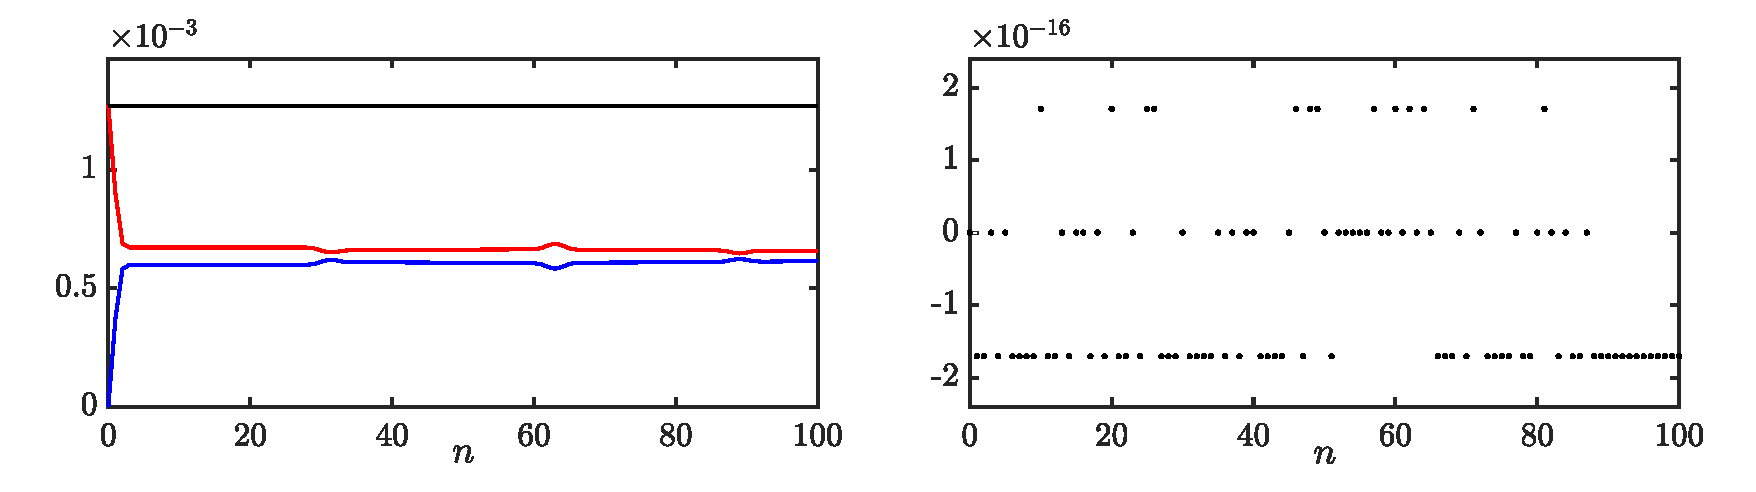
\includegraphics[width=\textwidth]{figures/resonators/brass/energyFirstOrder.eps}
        };
    
        \node[] (he) at (0.2,0.5) {\small $\mathfrak{h}_\text{e}$};

        \node[] (h) at (-5.75, 1) {\small $\mathfrak{h}$};
        \node[] (v) at (-5.75, 0.5) {\small $\color{red}\mathfrak{v}$};
        \node[] (t) at (-5.75, 0) {\small $\color{blue}\mathfrak{t}$};
    \end{tikzpicture}
      \caption{The kinetic (blue), potential (red), and total (black) energy of an implementation of the first-order system in Eq. \eqref{eq:firstOrderFDS} are plotted in the left panel. The right panel shows the normalised energy (according to Eq. \eqref{eq:normalisedEnergy}) and shows that the deviation of the energy is within machine precision. \label{fig:energyFirstOrder}}
\end{figure}

\subsection{Adding radiation}
\def\r{\text{r}}
\def\one{{(1)}}
Following \cite{Harrison2018}, radiation  can be added to the schemes using a circuit representation of the Levine and Schwinger radiation model (See Figure \ref{fig:circuit}). This section will provide a derivation \SWcomment[I'll actually move most of this to an appendix...]

\begin{figure}[h]
    \centering
    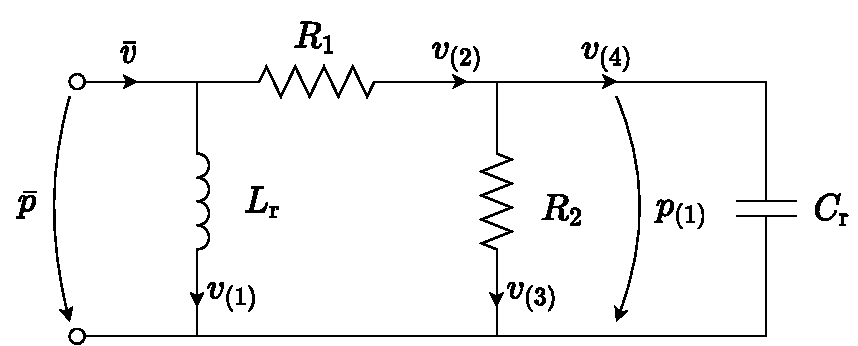
\includegraphics[width=0.7\textwidth]{figures/resonators/brass/circuit.pdf}
    \caption{The circuit representation of the Levine and Schwinger radiation model. \label{fig:circuit}}
\end{figure}

The system can be described as
\begin{subequations}\label{eq:barVPSystem}
    \begin{align}
        \bar v &= \mu_{t+}v_\one + \frac{1}{R_2}\mu_{t+}p_\one + C_\r \delta_{t+}p_\one,\label{eq:barV}\\
        \bar p &= L_\r \delta_{t+}v_\one,\label{eq:barP1}\\
        \bar p &= \left(1+\frac{R_1}{R_2}\right)\mu_{t+}p_\one+ R_1 C_\r\delta_{t+}p_\one\label{eq:barP2},
    \end{align}
\end{subequations}
where $\bar p^{n+1/2}$ and $\bar v^{n+1/2}$ are placed on the interleaved temporal grid and are related to the tube by
\begin{equation}\label{eq:barVars}
    \bar p = \mu_{t+}p^n_N, \quad \bar S_N \bar v = \mu_{x-}\left(S_{N+1/2}v_{N+1/2}^{n+1/2}\right).
\end{equation}
This can applied to the right boundary of the tube by evaluating Eq. \eqref{eq:pressureUpdate} at $l = N$
\begin{equation}
    p_N^{n+1} = p_N^n - \frac{\rho_0 c \lambda}{\bar{S}_N}\left(S_{N+1/2}v_{N+1/2}^{n+1/2}-S_{N-1/2}v_{N-1/2}^{n+1/2}\right),
\end{equation}
and, rewriting this to 
\begin{align}
    p_N^{n+1} &= p_N^n - \frac{\rho_0 c \lambda}{\bar{S}_N}\left(2\mu_{x-}\left(S_{N+1/2}v_{N+1/2}^{n+1/2}\right)-2S_{N-1/2}v_{N-1/2}^{n+1/2}\right)\nonumber,\\
    p_N^{n+1} &= p_N^n - \frac{2\rho_0 c \lambda}{\bar{S}_N}\left(\bar S_N \bar v-S_{N-1/2}v_{N-1/2}^{n+1/2}\right)\label{eq:preSolutP}.
\end{align}
A definition for $\bar v$ can then be found by first expanding Eq. \eqref{eq:barV} to 
\begin{equation}\label{eq:vBarExpanded}
    \bar v = \frac{1}{2}\left(v_\one^{n+1} + v_\one^n\right) + \left(\frac{1}{2R_2} + \frac{C_\r}{k}\right) p_\one^{n+1} +\left(\frac{1}{2R_2} - \frac{C_\r}{k}\right)p_\one^n.
\end{equation}
The goal is to make this definition solely dependent on the known values $v_\one^n$, $p_\one^n$ and $p_N^n$ and the unknown $p_N^{n+1}$ (as this can be obtained using Eq. \eqref{eq:preSolutP}).

Equation \eqref{eq:barP1} can be expanded to 
\begin{equation}\label{eq:voneNext}
    v_\one^{n+1} = \frac{k}{L_\r}\bar p + v_\one^n ,
\end{equation}
and Eq. \eqref{eq:barP2} to 
\begin{align*}
    &\bar p =\left(1+\frac{R_1}{R_2}\right)\mu_{t+}p_\one+ R_1 C_\r\delta_{t+}p_\one,\\
    &\bar p =\frac{1}{2}\left(1+\frac{R_1}{R_2}\right)\left(p_\one^{n+1} + p_\one^n\right) + \frac{R_1C_\r}{k}\left(p_\one^{n+1} - p_\one^n\right),\\
    \left(\frac{1}{2}+\frac{R_1}{2R_2} + \frac{R_1C_\r}{k}\right)&p_\one^{n+1} = \bar p + \left(\frac{R_1C_\r}{k} - \frac{1}{2} - \frac{R_1}{2R_2}\right)p_\one^n
\end{align*}
and finally solved for $p_\one^{n+1}$ as
\begin{equation}\label{eq:poneNext}
    p_\one^{n+1} = \underbrace{\left(\frac{2R_2k}{2R_1R_2C_\r + k(R_1 + R_2)}\right)}_{\zeta_1}\bar p + \underbrace{\left(\frac{2R_1R_2C_\r - k(R_1 + R_2)}{2R_1R_2C_\r + k(R_1 + R_2)}\right)}_{\zeta_2} p_\one^n .
\end{equation}
Equations \eqref{eq:voneNext} and \eqref{eq:poneNext} can then be substituted into Eq. \eqref{eq:vBarExpanded} and using the definition of $\bar p$ from Eq. \eqref{eq:barVars} yields
\begin{align}
    \bar v &= \frac{1}{2}\left(\frac{k}{L_\r}(\mu_{t+}p_N^n) + 2v_\one^n\right)+\left(\frac{1}{2R_2} + \frac{C_\r}{k}\right)\zeta_1\mu_{t+}p_N^n\nonumber \\
    & \qquad\qquad+ \left(\frac{1}{2R_2} + \frac{C_\r}{k}\right)\zeta_2p_\one^n + \left(\frac{1}{2R_2} - \frac{C_\r}{k}\right)p_\one^n\nonumber,\\
    \bar v &= \underbrace{\left(\frac{k}{2L_\r} + \frac{\zeta_1}{2R_2}+\frac{C_\r\zeta_1}{k}\right)}_{\zeta_3}\mu_{t+}p_N^n + v_\one^n + \underbrace{\left(\frac{\zeta_2+1}{2R_2} + \frac{C_\r\zeta_2 - C_\r}{k}\right)}_{\zeta_4}p_\one^n.
\end{align}
Finally, substituting this definition for $\bar v$ into Eq. \eqref{eq:preSolutP} yields
\begin{align}
    p_N^{n+1} &= p_N^n - \frac{2\rho_0c\lambda}{\bar S_N}\left(\bar S_N
    \left[\zeta_3\left(\frac{p_N^{n+1} + p_N^n}{2}\right) + v_\one^n + \zeta_4p_\one^n\right] - S_{N-1/2}v_{N-1/2}^{n+1/2}\right)\nonumber\\
    p_N^{n+1} &= p_N^n - \rho_0c\lambda\left(\zeta_3(p_N^{n+1} + p_N^n) + 2(v_\one^n + \zeta_4p_\one^n)-\frac{2S_{N-1/2}v_{N-1/2}^{n+1/2}}{\bar S_N}\right)\nonumber
\end{align}
and yields a definition for $p_N^{n+1}$ based on known values of the system 
\begin{equation}
    p_N^{n+1} = \frac{1 - \rho_0c\lambda\zeta_3}{1+\rho_0c\lambda\zeta_3}p_N^n - \frac{2\rho_0c\lambda}{1+\rho_0c\lambda\zeta_3} \left( v_\one^n+\zeta_4p_\one^n - \frac{S_{N-1/2}v_{N-1/2}^{n+1/2}}{\bar S_N}\right).
\end{equation}
\subsection{Energy}
\SWcomment[not done yet...]
Recalling the condition at the right boundary from \eqref{eq:firstOrderRightBoundary}
\begin{equation}
    \mathfrak{b}_\r = (\mu_{t+}p_N)\underbrace{\mu_{x+}(S_{N-1/2}v_{N-1/2})}_{\mu_{x-}S_{N+1/2}v_{N+1/2}},
\end{equation}
using Eq. \eqref{eq:barVars} one can rewrite this to
\begin{equation}
    \mathfrak{b}_\r = \bar p\bar S_N\bar v.
\end{equation}
then we can 